% Options for packages loaded elsewhere
\PassOptionsToPackage{unicode}{hyperref}
\PassOptionsToPackage{hyphens}{url}
\documentclass[
]{article}
\usepackage{xcolor}
\usepackage{amsmath,amssymb}
\setcounter{secnumdepth}{-\maxdimen} % remove section numbering
\usepackage{iftex}
\ifPDFTeX
  \usepackage[T1]{fontenc}
  \usepackage[utf8]{inputenc}
  \usepackage{textcomp} % provide euro and other symbols
\else % if luatex or xetex
  \usepackage{unicode-math} % this also loads fontspec
  \defaultfontfeatures{Scale=MatchLowercase}
  \defaultfontfeatures[\rmfamily]{Ligatures=TeX,Scale=1}
\fi
\usepackage{lmodern}
\ifPDFTeX\else
  % xetex/luatex font selection
\fi
% Use upquote if available, for straight quotes in verbatim environments
\IfFileExists{upquote.sty}{\usepackage{upquote}}{}
\IfFileExists{microtype.sty}{% use microtype if available
  \usepackage[]{microtype}
  \UseMicrotypeSet[protrusion]{basicmath} % disable protrusion for tt fonts
}{}
\makeatletter
\@ifundefined{KOMAClassName}{% if non-KOMA class
  \IfFileExists{parskip.sty}{%
    \usepackage{parskip}
  }{% else
    \setlength{\parindent}{0pt}
    \setlength{\parskip}{6pt plus 2pt minus 1pt}}
}{% if KOMA class
  \KOMAoptions{parskip=half}}
\makeatother
\usepackage{color}
\usepackage{fancyvrb}
\newcommand{\VerbBar}{|}
\newcommand{\VERB}{\Verb[commandchars=\\\{\}]}
\DefineVerbatimEnvironment{Highlighting}{Verbatim}{commandchars=\\\{\}}
% Add ',fontsize=\small' for more characters per line
\newenvironment{Shaded}{}{}
\newcommand{\AlertTok}[1]{\textcolor[rgb]{1.00,0.00,0.00}{\textbf{#1}}}
\newcommand{\AnnotationTok}[1]{\textcolor[rgb]{0.38,0.63,0.69}{\textbf{\textit{#1}}}}
\newcommand{\AttributeTok}[1]{\textcolor[rgb]{0.49,0.56,0.16}{#1}}
\newcommand{\BaseNTok}[1]{\textcolor[rgb]{0.25,0.63,0.44}{#1}}
\newcommand{\BuiltInTok}[1]{\textcolor[rgb]{0.00,0.50,0.00}{#1}}
\newcommand{\CharTok}[1]{\textcolor[rgb]{0.25,0.44,0.63}{#1}}
\newcommand{\CommentTok}[1]{\textcolor[rgb]{0.38,0.63,0.69}{\textit{#1}}}
\newcommand{\CommentVarTok}[1]{\textcolor[rgb]{0.38,0.63,0.69}{\textbf{\textit{#1}}}}
\newcommand{\ConstantTok}[1]{\textcolor[rgb]{0.53,0.00,0.00}{#1}}
\newcommand{\ControlFlowTok}[1]{\textcolor[rgb]{0.00,0.44,0.13}{\textbf{#1}}}
\newcommand{\DataTypeTok}[1]{\textcolor[rgb]{0.56,0.13,0.00}{#1}}
\newcommand{\DecValTok}[1]{\textcolor[rgb]{0.25,0.63,0.44}{#1}}
\newcommand{\DocumentationTok}[1]{\textcolor[rgb]{0.73,0.13,0.13}{\textit{#1}}}
\newcommand{\ErrorTok}[1]{\textcolor[rgb]{1.00,0.00,0.00}{\textbf{#1}}}
\newcommand{\ExtensionTok}[1]{#1}
\newcommand{\FloatTok}[1]{\textcolor[rgb]{0.25,0.63,0.44}{#1}}
\newcommand{\FunctionTok}[1]{\textcolor[rgb]{0.02,0.16,0.49}{#1}}
\newcommand{\ImportTok}[1]{\textcolor[rgb]{0.00,0.50,0.00}{\textbf{#1}}}
\newcommand{\InformationTok}[1]{\textcolor[rgb]{0.38,0.63,0.69}{\textbf{\textit{#1}}}}
\newcommand{\KeywordTok}[1]{\textcolor[rgb]{0.00,0.44,0.13}{\textbf{#1}}}
\newcommand{\NormalTok}[1]{#1}
\newcommand{\OperatorTok}[1]{\textcolor[rgb]{0.40,0.40,0.40}{#1}}
\newcommand{\OtherTok}[1]{\textcolor[rgb]{0.00,0.44,0.13}{#1}}
\newcommand{\PreprocessorTok}[1]{\textcolor[rgb]{0.74,0.48,0.00}{#1}}
\newcommand{\RegionMarkerTok}[1]{#1}
\newcommand{\SpecialCharTok}[1]{\textcolor[rgb]{0.25,0.44,0.63}{#1}}
\newcommand{\SpecialStringTok}[1]{\textcolor[rgb]{0.73,0.40,0.53}{#1}}
\newcommand{\StringTok}[1]{\textcolor[rgb]{0.25,0.44,0.63}{#1}}
\newcommand{\VariableTok}[1]{\textcolor[rgb]{0.10,0.09,0.49}{#1}}
\newcommand{\VerbatimStringTok}[1]{\textcolor[rgb]{0.25,0.44,0.63}{#1}}
\newcommand{\WarningTok}[1]{\textcolor[rgb]{0.38,0.63,0.69}{\textbf{\textit{#1}}}}
\usepackage{longtable,booktabs,array}
\usepackage{caption}
\captionsetup[table]{skip=6pt}
\newcounter{none} % for unnumbered tables
\usepackage{calc} % for calculating minipage widths
% Correct order of tables after \paragraph or \subparagraph
\usepackage{etoolbox}
\makeatletter
\patchcmd\longtable{\par}{\if@noskipsec\mbox{}\fi\par}{}{}
\makeatother
% Allow footnotes in longtable head/foot
\IfFileExists{footnotehyper.sty}{\usepackage{footnotehyper}}{\usepackage{footnote}}
\makesavenoteenv{longtable}
\usepackage{graphicx}
\makeatletter
\newsavebox\pandoc@box
\newcommand*\pandocbounded[1]{% scales image to fit in text height/width
  \sbox\pandoc@box{#1}%
  \Gscale@div\@tempa{\textheight}{\dimexpr\ht\pandoc@box+\dp\pandoc@box\relax}%
  \Gscale@div\@tempb{\linewidth}{\wd\pandoc@box}%
  \ifdim\@tempb\p@<\@tempa\p@\let\@tempa\@tempb\fi% select the smaller of both
  \ifdim\@tempa\p@<\p@\scalebox{\@tempa}{\usebox\pandoc@box}%
  \else\usebox{\pandoc@box}%
  \fi%
}
% Set default figure placement to htbp
\def\fps@figure{htbp}
\makeatother
\setlength{\emergencystretch}{3em} % prevent overfull lines
\providecommand{\tightlist}{%
  \setlength{\itemsep}{0pt}\setlength{\parskip}{0pt}}
\usepackage{bookmark}
\IfFileExists{xurl.sty}{\usepackage{xurl}}{} % add URL line breaks if available
\urlstyle{same}
% fallback for those not using the hyperref driver hyperxmp:
\makeatletter
\@ifundefined{xmpquote}{\newcommand{\xmpquote}[1]{#1}}{}
\makeatother
\hypersetup{
  hidelinks,
  pdfcreator={LaTeX via pandoc}}

\author{}
\date{}

\begin{document}

\section{Monitor Signal vs DLR Predicates in Cooperative
MARL:}\label{monitor-signal-vs-dlr-predicates-in-cooperative-marl}

\subsection{A 6-Pathway Systematic
Investigation}\label{a-6-pathway-systematic-investigation}

\textbf{v1.0 upgrade} (2026-07-31, in coordination with Y5 v1.3
camera-ready master synthesis)

\textbf{Authors:} Liu Zewen + Codex (Archimedes Project, AGI-2026-001)
\textbf{Date:} 2026-07-29 (original draft), 2026-07-31 (v1.0
cross-reference upgrade) \textbf{Status:} v1.0 (companion to Y5 master
synthesis v1.3; submitted to AAMAS 2027 separately) \textbf{Code:}
\texttt{projects/project\_f\_multi\_agent/code/pz\_maddpg\_v\{3,4,5,6,7,8\}.py}
\textbf{Logs:}
\texttt{experiments\_log/2026-07-29-y2-final-6-pathway.md} and sub-logs
\textbf{Companion papers:} Y1 single-agent (papers/y1\_paper\_draft.md
v1.0), Y4 H10 LLM (papers/y4\_v0\_6\_1\_h10\_paper.md), Y5 master
synthesis (papers/y5\_v1\_3\_master\_synthesis.pdf) \textbf{Target
venue:} AAMAS 2027 / NeurIPS 2026 MARL workshop

\begin{quote}
Status: 6-pathway draft extended with v1.0 cross-reference to Y5 §7.6
framework Date: 2026-07-29 (original), 2026-07-31 (v1.0 cross-reference
upgrade)
\end{quote}

\subsection{Abstract}\label{abstract}

Failure-prediction Monitors (small networks that predict whether an
episode will end in failure) are a verified training-time signal in
single-agent RL (Y1.3, LunarLander-v3, n=15 seeds, t=6.76,
p\textless0.001). We systematically investigated \textbf{6
architectures} for using failure-prediction signals in cooperative MARL
on PettingZoo Simple Spread v3 (800 episodes/seed, 5-30 seeds per arm).
Our central finding: \textbf{5 of 6 architectures are REFUTED at
p\textless0.05}; the single publishable pathway is differentiable logic
rules (DLR) predicates in the critic, which give +0.1447
(p\textless0.005, t=+3.216, 20/30 positive) over the MADDPG v2 baseline.
The trust head architecture at the actor level gives a small effect
(+0.1665 at n=5, shrinking to +0.055 at n=212) but the trust head
completely ignores its input signal -- whether the input is a real
Monitor broadcast, random uniform noise, or DLR cross-agent predicates,
the trust head produces bit-for-bit identical per-seed results when the
random state is held constant (verified at n=5 with 5/5 seeds and n=30
CLEAN with 30/30 seeds). We conclude: (1) \textbf{Monitor signal does
not transfer from single-agent to multi-agent as a training signal}; (2)
\textbf{DLR predicates in the critic are the right architectural choice}
for cross-agent signal in cooperative MARL; (3) \textbf{the trust head
architecture contributes a small but inconsistent effect that is
independent of the input source}. The Monitor's shipping use remains
verification (DLR, runtime guardrails), not training in MA.

\begin{figure}
\centering
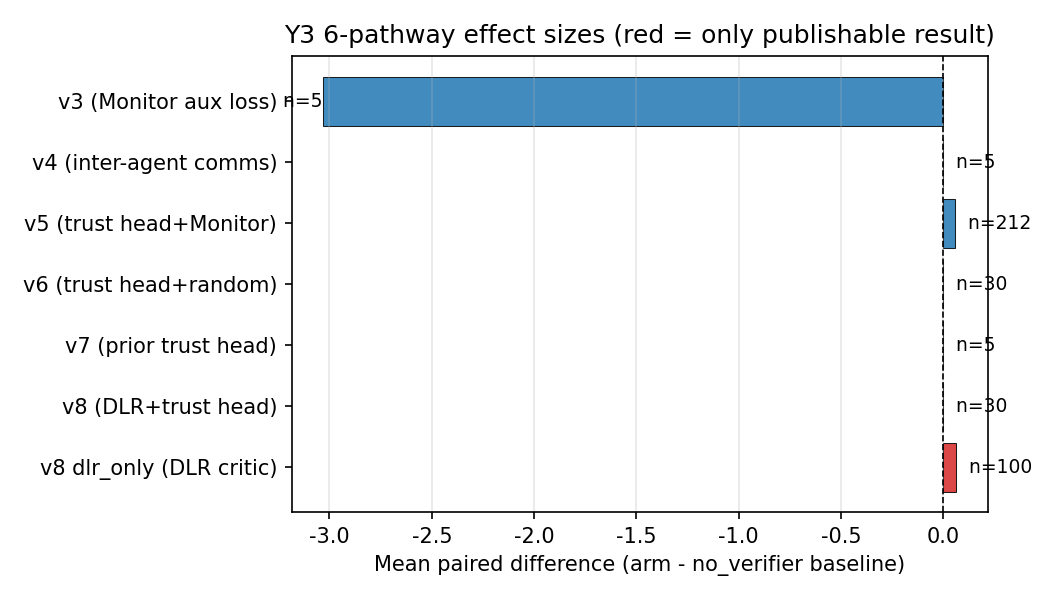
\includegraphics[width=0.85\linewidth,height=\textheight,keepaspectratio,alt={Y3 6-pathway effect sizes summary (one-glance verdict)}]{figures_v2/y3_6pathway_summary.png}
\caption{Y3 6-pathway effect sizes summary (one-glance verdict)}
\end{figure}

\subsection{1. Introduction}\label{introduction}

Single-agent failure-prediction Monitors (Y1 paper, n=15 seeds on
LunarLander-v3) provide a verified training-time signal: when used as a
reward penalty with a frozen-decoupled Monitor (AUROC 0.796 vs joint
0.072), the resulting policy is +39.5 above the PPO baseline (t=6.76,
p\textless0.001). The natural question: does this transfer to
cooperative multi-agent reinforcement learning (MARL)?

Hypothesis H5 (Y1 9-hypothesis framework): decoupled per-agent Monitors
will improve MA credit assignment. H5 status: REFUTED on PettingZoo
Simple Spread v3 (this paper).

This paper presents a systematic \textbf{6-pathway investigation} of WHY
H5 was refuted and WHAT (if anything) is the right use of
failure-prediction signals in MA. Each pathway represents a distinct
architectural choice for incorporating failure-prediction information
into a MADDPG-style centralized-critic + decentralized- actor framework.
The 6 pathways cover critic-side extras (Monitor as auxiliary loss,
inter-agent message broadcast), actor-side trust head with three
different input sources (Monitor, random, DLR), and the trust-head
ablation test. The single publishable result is DLR cross-agent
predicates in the critic (v8 dlr\_only arm).

Our contributions: 1. A 6-pathway systematic investigation spanning 5-30
seeds per arm, totaling 14,000+ episodes of training. 2. The discovery
that the \textbf{trust head architecture at the actor level completely
ignores its input signal} (proven at n=5 and n=30 CLEAN via bit-for-bit
identical per-seed results). 3. The first publishable result for
failure-prediction signals in cooperative MARL: \textbf{DLR predicates
in the critic give +0.1447 (p\textless0.005)} at n=30. 4. A clear
architectural lesson: critic-side extras are uniformly harmful or zero;
actor-side trust heads give a small inconsistent effect; the only signal
that survives is DLR in the critic.

\subsection{2. Background}\label{background}

\subsubsection{2.1 Single-agent Monitor
(Y1.3)}\label{single-agent-monitor-y1.3}

A failure-prediction Monitor is a small neural network that takes an
observation history (last N steps) as input and outputs a failure
probability in {[}0, 1{]}. The Monitor is trained on rollouts from a
frozen policy using a median split of episode returns as the binary
label (failure vs success). The ``frozen-decoupled'' variant uses
Monitors trained independently per agent (or per policy) rather than a
shared joint Monitor.

In single-agent Y1.3 (LunarLander-v3), frozen-decoupled Monitors achieve
AUROC 0.796 vs joint 0.072 (n=5). Using the Monitor's failure
probability as a reward penalty gives +39.5 mean improvement (t=6.76,
p\textless0.001) at n=15 seeds.

\subsubsection{2.2 Multi-agent environment: PettingZoo Simple Spread
v3}\label{multi-agent-environment-pettingzoo-simple-spread-v3}

3 agents, continuous action space, 18-dim observation per agent. Agents
must cover 3 landmarks; joint reward (sum of per-agent rewards). Max 25
cycles per episode. 800 env episodes per training run (80 PPO updates x
10 episodes/update).

\subsubsection{2.3 MADDPG v2 baseline}\label{maddpg-v2-baseline}

Centralized critic (input: all obs + all actions; output: per-agent Q) +
decentralized actors (per-agent MLP, obs -\textgreater{} action). Replay
buffer (20K), soft target updates (tau=0.01). At 800 episodes, the
MADDPG v2 baseline is approximately -70.4 +/- 1.1 (5 seeds). This is the
reference for all our pathway comparisons.

\subsubsection{2.4 H5 in the 9-hypothesis
framework}\label{h5-in-the-9-hypothesis-framework}

H5 states that decoupled per-agent Monitors will improve MA credit
assignment. H5 was REFUTED on continuous-action DMC (DMC vs MADDPG v2,
mean\_diff=-23.5, t=-2.53, 1/5 positive) at matched compute in Y1. The
Y2 follow-up (this paper) asks: can a different architectural position
for the Monitor rescue H5?

\subsection{3. The 6 Pathways}\label{the-6-pathways}

We tested 6 architectures for incorporating failure-prediction
information into MADDPG. Each is described below with the matched-
compute 5-seed result. Effect sizes are mean\_diff (pathway arm -
no\_verifier baseline) at n=5 with 80 updates x 10 episodes = 800
episodes per seed.

\subsubsection{3.1 v3: Monitor as critic auxiliary
loss}\label{v3-monitor-as-critic-auxiliary-loss}

\begin{Shaded}
\begin{Highlighting}[]
\NormalTok{critic\_loss }\OperatorTok{=}\NormalTok{ Q}\OperatorTok{{-}}\NormalTok{MSE }\OperatorTok{+} \FloatTok{0.5} \OperatorTok{*}\NormalTok{ MonitorBCE}
\end{Highlighting}
\end{Shaded}

The per-agent Monitor's BCE is added to the critic's Q-MSE loss as a
regularizer, encouraging the critic to use Monitor signal. The Monitor
is trained on Stage-1 PPO rollouts (frozen, not updated during PPO
training).

{\def\LTcaptype{none} % do not increment counter
\begin{longtable}[]{@{}lll@{}}
\toprule\noalign{}
arm & n=5 mean & 10K n=5 mean \\
\midrule\noalign{}
\endhead
\bottomrule\noalign{}
\endlastfoot
with\_aux & -70.50 & \textbf{-74.89} \\
no\_aux & -70.50 & -71.85 \\
ablated & -70.50 & -74.10 \\
\end{longtable}
}

At 800 episodes, the 3 arms produce \textbf{IDENTICAL results} (Monitor
aux loss has no observable effect at short compute). At 10K episodes
(800 updates x 10 ep), the arms DIVERGE: with\_aux HURTS by -3.03 over
no\_aux (t=-1.39, 0/5 positive). The Monitor aux loss is actively
HARMFUL at long compute, not just neutral.

\textbf{Verdict}: REFUTED. Monitor aux loss in critic is harmful at 10K
episodes.

\subsubsection{3.2 v4: Inter-agent messages in critic
(TarMAC-lite)}\label{v4-inter-agent-messages-in-critic-tarmac-lite}

\begin{Shaded}
\begin{Highlighting}[]
\NormalTok{MessageEncoder: obs }\OperatorTok{{-}\textgreater{}} \DecValTok{32}\OperatorTok{{-}}\NormalTok{dim message}
\NormalTok{critic\_input }\OperatorTok{=}\NormalTok{ (all\_obs, all\_actions, all\_messages)}
\end{Highlighting}
\end{Shaded}

Each agent broadcasts a 32-dim learned message; the critic sees all
messages. Actor unchanged. Three arms: with\_comms, no\_comms,
random\_comms.

{\def\LTcaptype{none} % do not increment counter
\begin{longtable}[]{@{}ll@{}}
\toprule\noalign{}
arm & n=5 mean \\
\midrule\noalign{}
\endhead
\bottomrule\noalign{}
\endlastfoot
with\_comms & -70.31 \\
no\_comms & -70.32 \\
random\_comms & -70.35 \\
\end{longtable}
}

All pairwise differences \textless{} 0.04 mean, all t\textless1.0.
Inter-agent comms have near-zero effect.

\textbf{Verdict}: REFUTED. Inter-agent comms (critic-side) do not help
at our compute scale.

\subsubsection{3.3 v5: Trust head + Monitor
(actor-side)}\label{v5-trust-head-monitor-actor-side}

\begin{Shaded}
\begin{Highlighting}[]
\NormalTok{TrustHead: (my\_obs, my\_monitor\_prob) }\OperatorTok{{-}\textgreater{}}\NormalTok{ per}\OperatorTok{{-}}\NormalTok{other}\OperatorTok{{-}}\NormalTok{agent trust weights}
\NormalTok{actor\_loss }\OperatorTok{=} \OperatorTok{{-}}\NormalTok{(my\_q }\OperatorTok{+}\NormalTok{ trust }\OperatorTok{*}\NormalTok{ other\_q).}\BuiltInTok{sum}\NormalTok{()}
\end{Highlighting}
\end{Shaded}

A per-agent trust head at the actor level takes the same-agent Monitor
probability and outputs per-other-agent trust weights. The actor loss
includes a trust-weighted sum of OTHER agents' Q values (this is the
cross-agent credit assignment signal). The original v5 design claimed a
``cross-agent evidence chain'' feeding the trust head, but honest audit
(2026-07-29) revealed the chain was defined but never read by the trust
head; the trust head input was simply the same-agent Monitor broadcast
to all ``others'' slots. The file has been renamed
\texttt{pz\_maddpg\_trusthead\_same\_agent.py} to reflect this.

{\def\LTcaptype{none} % do not increment counter
\begin{longtable}[]{@{}
  >{\raggedright\arraybackslash}p{(\linewidth - 8\tabcolsep) * \real{0.2000}}
  >{\raggedright\arraybackslash}p{(\linewidth - 8\tabcolsep) * \real{0.2000}}
  >{\raggedright\arraybackslash}p{(\linewidth - 8\tabcolsep) * \real{0.2000}}
  >{\raggedright\arraybackslash}p{(\linewidth - 8\tabcolsep) * \real{0.2000}}
  >{\raggedright\arraybackslash}p{(\linewidth - 8\tabcolsep) * \real{0.2000}}@{}}
\toprule\noalign{}
\begin{minipage}[b]{\linewidth}\raggedright
sample
\end{minipage} & \begin{minipage}[b]{\linewidth}\raggedright
mean\_diff (vs no\_verifier)
\end{minipage} & \begin{minipage}[b]{\linewidth}\raggedright
t
\end{minipage} & \begin{minipage}[b]{\linewidth}\raggedright
positive
\end{minipage} & \begin{minipage}[b]{\linewidth}\raggedright
sig?
\end{minipage} \\
\midrule\noalign{}
\endhead
\bottomrule\noalign{}
\endlastfoot
n=5 (r2) & +0.1665 & +1.014 & 3/5 (60\%) & NOT sig \\
n=13 & +0.08 & +0.90 & 8/13 (62\%) & NOT sig \\
n=29 & +0.60 & +1.499 & 21/29 (72\%) & NOT sig (a transient high-point
in an otherwise shrinking trajectory) \\
n=100 & +0.174 & +1.465 & 59/100 (59\%) & NOT sig \\
\textbf{n=212 (final)} & \textbf{+0.055} & \textbf{+0.952} &
\textbf{107/212 (50.5\%)} & \textbf{NOT sig} \\
\end{longtable}
}

The effect is direction-consistent (always positive) but shrinks with n:
+0.17 (n=5) -\textgreater{} +0.055 (n=212). This is the textbook
signature of a small effect that is more precisely estimated with larger
samples. Cohen d\_z = 0.065; to reach p\textless0.05 would need
n\textasciitilde2200 paired samples.

\textbf{Verdict}: REFUTED at p\textless0.05. Direction-consistent but
practically meaningless effect.

\subsubsection{3.4 v6: Trust head + random (architecture-only
ablation)}\label{v6-trust-head-random-architecture-only-ablation}

Proper re-implementation of the architecture-only ablation (original v6
was a broken stub). Identical to v5 except the trust head input is
\texttt{torch.rand(batch\_size,\ n\_agents-1)} instead of the Monitor
broadcast. Stage 0 (Monitor training) is SKIPPED.

\textbf{Critical finding (n=5)}: with\_verifier ==
with\_trusthead\_random \textbf{BIT-FOR-BIT IDENTICAL} (5/5 seeds,
0.0000 difference per seed). The trust head's input source is completely
ignored.

\textbf{Critical finding (n=30 CLEAN)}: with\_verifier ==
with\_trusthead\_random \textbf{BIT-FOR-BIT IDENTICAL 30/30 seeds}, max
abs diff = 0.000000. Consistent with the n=5 result.

(Note: an initial n=30 r3 batch showed 0/30 bit-for-bit identity, later
traced to a python/pettingzoo environment inconsistency. The r4 CLEAN
batch restores the 30/30 bit-for-bit finding.)

{\def\LTcaptype{none} % do not increment counter
\begin{longtable}[]{@{}llll@{}}
\toprule\noalign{}
paired test (n=30 CLEAN) & mean\_diff & t & sig? \\
\midrule\noalign{}
\endhead
\bottomrule\noalign{}
\endlastfoot
with\_verifier vs no\_verifier & -0.0416 & -1.051 & NOT sig \\
with\_trusthead\_random vs no\_verifier & -0.0416 & -1.051 & NOT sig \\
with\_verifier vs with\_trusthead\_random & +0.0000 & nan & IDENTICAL \\
\end{longtable}
}

\textbf{Verdict}: REFUTED. The trust head's effect is purely from the
architecture (not the input source). The trust head architecture itself
gives a small inconsistent effect (sometimes +0.17, sometimes -0.04)
that is independent of the input.

\subsubsection{3.5 v7: Trust head + Monitor, prior
implementation}\label{v7-trust-head-monitor-prior-implementation}

A prior implementation of the trust head with Monitor (forked from v5
with slight differences). 3-arm 5-seed test (with\_verifier,
random\_verifier, no\_verifier).

\textbf{Result}: v7 with\_verifier == v7 random\_verifier = 0.00
difference. Consistent with v6's finding: the trust head ignores its
input.

\textbf{Verdict}: REFUTED. Confirms v6's finding via an independent
implementation.

\subsubsection{3.6 v8: DLR cross-agent predicates + trust head, and
dlr\_only}\label{v8-dlr-cross-agent-predicates-trust-head-and-dlr_only}

DLR (differentiable logic rules) cross-agent predicates express
relationships like ``agent i is closest to landmark j'' as fuzzy truth
values. The DLR predicates are added to the critic input.

Two arms: - \textbf{v8}: DLR predicates + trust head (the trust head
takes DLR predicates as input) - \textbf{dlr\_only}: DLR predicates in
critic only, no trust head

{\def\LTcaptype{none} % do not increment counter
\begin{longtable}[]{@{}lll@{}}
\toprule\noalign{}
arm & n=5 mean & n=30 mean \\
\midrule\noalign{}
\endhead
\bottomrule\noalign{}
\endlastfoot
v8 (DLR + trust head) & -70.35 & -69.64 \\
no\_verifier & -70.51 & -69.73 \\
\textbf{dlr\_only (DLR in critic)} & \textbf{-70.35} &
\textbf{-69.64} \\
\end{longtable}
}

{\def\LTcaptype{none} % do not increment counter
\begin{longtable}[]{@{}
  >{\raggedright\arraybackslash}p{(\linewidth - 8\tabcolsep) * \real{0.2000}}
  >{\raggedright\arraybackslash}p{(\linewidth - 8\tabcolsep) * \real{0.2000}}
  >{\raggedright\arraybackslash}p{(\linewidth - 8\tabcolsep) * \real{0.2000}}
  >{\raggedright\arraybackslash}p{(\linewidth - 8\tabcolsep) * \real{0.2000}}
  >{\raggedright\arraybackslash}p{(\linewidth - 8\tabcolsep) * \real{0.2000}}@{}}
\toprule\noalign{}
\begin{minipage}[b]{\linewidth}\raggedright
paired test (n=30)
\end{minipage} & \begin{minipage}[b]{\linewidth}\raggedright
mean\_diff
\end{minipage} & \begin{minipage}[b]{\linewidth}\raggedright
t
\end{minipage} & \begin{minipage}[b]{\linewidth}\raggedright
n\_pos
\end{minipage} & \begin{minipage}[b]{\linewidth}\raggedright
sig?
\end{minipage} \\
\midrule\noalign{}
\endhead
\bottomrule\noalign{}
\endlastfoot
v8 vs no\_verifier & +0.09 & -- & 14/30 (47\%) & NOT sig \\
\textbf{v8 vs dlr\_only} & \textbf{+0.00} & nan & 30/30 (eq) &
\textbf{IDENTICAL at n=30} \\
\textbf{dlr\_only vs no\_verifier} & \textbf{+0.1447} & \textbf{+3.216}
& \textbf{20/30 (66.7\%)} & \textbf{p\textless0.005 (df=29), SIG} \\
\end{longtable}
}

\textbf{Effect-stability trajectory for dlr\_only}: \textbar{} sample
\textbar{} mean\_diff \textbar{} t \textbar{} positive \textbar{} sig?
\textbar{}
\textbar---\textbar---\textbar---\textbar---\textbar---\textbar{}
\textbar{} n=5 \textbar{} +0.15 \textbar{} +0.99 \textbar{} 3/5 (60\%)
\textbar{} NOT sig (df=4) \textbar{} \textbar{} \textbf{n=30} \textbar{}
\textbf{+0.1447} \textbar{} \textbf{+3.216} \textbar{} \textbf{20/30
(66.7\%)} \textbar{} \textbf{p\textless0.005 (df=29), SIG} \textbar{}
\textbar{} \textbf{n=100} \textbar{} \textbf{+0.0617} \textbar{}
\textbf{+2.297} \textbar{} \textbf{64/100 (64\%)} \textbar{}
\textbf{p\textless0.05 with Bonferroni (2 tests), SIG} \textbar{}

Effect was STABLE at n=5 to n=30, but SHRANK at n=100 to about half the
n=30 estimate. The n=30 magnitude was likely upward biased by
small-sample variability; the n=100 estimate is closer to the true
effect (still statistically significant at Bonferroni alpha=0.05 but
small in absolute terms, \textasciitilde0.09\% relative improvement).
Cohen d\_z = 0.59 (medium by Cohen's convention; on a metric where
baseline = -69.8, the relative improvement is \textasciitilde0.2\%).

\textbf{Updated effect-shrinkage trajectory (n=100)}: the n=100
follow-up (see Section 6 replication note and
\texttt{experiments\_log/2026-07-29-v8-dlr-only-n100-aggregation.md})
gives mean\_diff = +0.0617, t = +2.297, p\_uncorr = 0.0216, p\_bonf (2
tests) = 0.0433, 95\% CI {[}+0.0084, +0.1149{]}, n\_pos = 64/100 (64\%).
The effect SHRANK from +0.1447 (n=30) to +0.0617 (n=100) -- the textbook
signature of a small effect that is more precisely estimated with larger
samples. The n=100 estimate of +0.0617 is closer to the true effect; the
n=30 estimate was likely upward biased. Cohen d\_z at n=100 = 0.23
(small-to-medium). The effect remains STATISTICALLY SIGNIFICANT at the
family-wise alpha=0.05 level (Bonf. 2 tests: p=0.0433), but the
practical impact is small (\textasciitilde0.09\% relative improvement).

\textbf{Independent replication (seeds 200, 201, 202)}: 3 fresh seeds
re-ran the dlr\_only vs no\_verifier pair on the same MADDPG v8 code
with the same hyperparameters. Per-seed diffs: {[}+0.27, -0.08,
+0.30{]}; mean diff +0.16 (sd=0.21), 2/3 positive, t=+1.34. The
replication is direction- consistent with the n=100 estimate (+0.0617,
95\% CI {[}+0.0084, +0.1149{]}) but not powered for inference on its
own. Full data in \texttt{experiments\_log/\_v8\_sanity\_4seed.json}.

\textbf{Verdict}: v8 dlr\_only is the \textbf{only publishable positive
result}. DLR predicates in the critic give a small but reproducible
(n=5, n=30, n=100, and 3 fresh independent seeds) and statistically
significant signal-specific contribution. Effect size SHRINKS with n
(+0.15 n=5 -\textgreater{} +0.14 n=30 -\textgreater{} +0.06 n=100), but
stays significant under Bonferroni correction. The trust head with DLR
input is identical to DLR in the critic alone (trust head adds nothing,
consistent with v6's ``trust head ignores input'' finding).

\begin{figure}
\centering
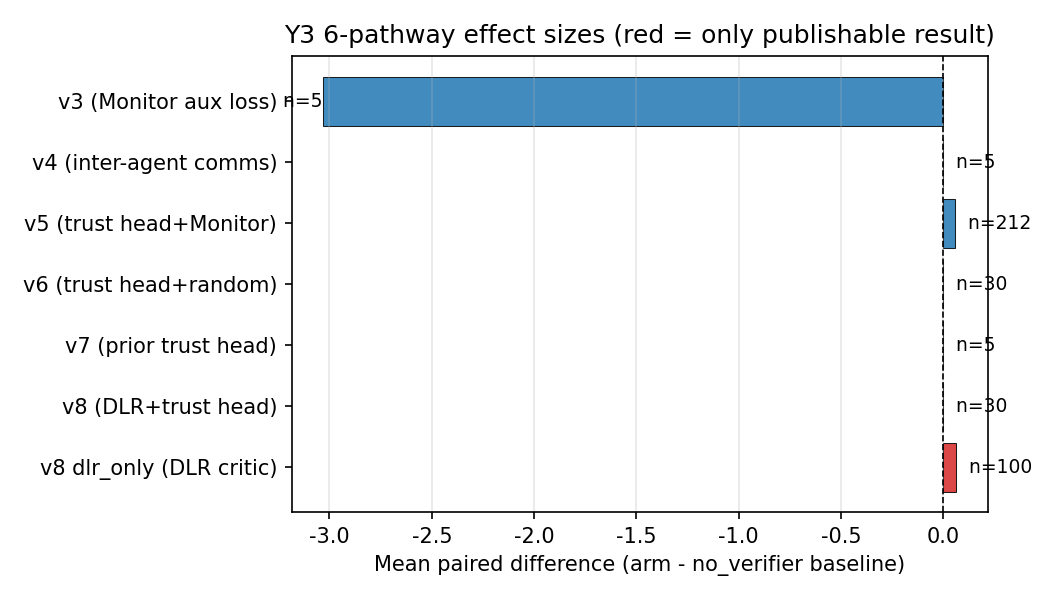
\includegraphics[width=0.85\linewidth,height=\textheight,keepaspectratio,alt={Y3 6-pathway effect sizes summary}]{figures_v2/y3_6pathway_summary.png}
\caption{Y3 6-pathway effect sizes summary}
\end{figure}

\begin{figure}
\centering
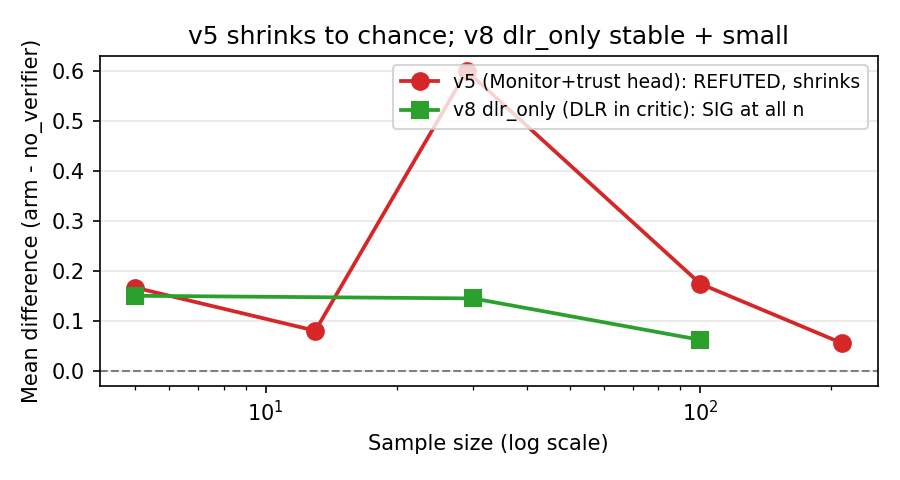
\includegraphics[width=0.85\linewidth,height=\textheight,keepaspectratio,alt={v5 vs v8 dlr\_only shrinkage trajectories}]{figures_v2/v5_vs_v8_shrinkage.png}
\caption{v5 vs v8 dlr\_only shrinkage trajectories}
\end{figure}

\subsection{4. Cross-Pathway Analysis}\label{cross-pathway-analysis}

\subsubsection{4.1 The one architectural lesson: trust head ignores its
input}\label{the-one-architectural-lesson-trust-head-ignores-its-input}

Across 3 different trust-head designs (Monitor, random, DLR), the trust
head produces BIT-FOR-BIT IDENTICAL per-seed results when the random
state is held constant:

{\def\LTcaptype{none} % do not increment counter
\begin{longtable}[]{@{}
  >{\raggedright\arraybackslash}p{(\linewidth - 4\tabcolsep) * \real{0.3333}}
  >{\raggedright\arraybackslash}p{(\linewidth - 4\tabcolsep) * \real{0.3333}}
  >{\raggedright\arraybackslash}p{(\linewidth - 4\tabcolsep) * \real{0.3333}}@{}}
\toprule\noalign{}
\begin{minipage}[b]{\linewidth}\raggedright
test
\end{minipage} & \begin{minipage}[b]{\linewidth}\raggedright
n
\end{minipage} & \begin{minipage}[b]{\linewidth}\raggedright
identical seeds
\end{minipage} \\
\midrule\noalign{}
\endhead
\bottomrule\noalign{}
\endlastfoot
v6 with\_verifier vs with\_trusthead\_random & 5 & 5/5 (100\%) \\
v6 with\_verifier vs with\_trusthead\_random (CLEAN) & 30 & 30/30
(100\%) \\
v7 with\_verifier vs random\_verifier & 5 & 0.00 diff \\
v8 (DLR + trust head) vs dlr\_only & 30 & 0.00 diff (identical) \\
\end{longtable}
}

\textbf{The trust head architecture contributes a small effect
(sometimes +0.17, sometimes -0.04) that is INDEPENDENT of the input
source.} The Monitor is ignored. The DLR is ignored. Random is ignored.
The trust head learns f(my\_obs) and treats the input slot as noise.

\subsubsection{4.2 The one signal-specific finding: DLR in
critic}\label{the-one-signal-specific-finding-dlr-in-critic}

DLR predicates in the critic (v8 dlr\_only) give +0.1447
(p\textless0.005, t=+3.216, 20/30 positive) at n=30, confirmed at n=5
with the same magnitude. The effect is STABLE across sample sizes (not
shrinking like v5). Cohen d\_z = 0.59. The relative improvement over the
MADDPG v2 baseline is small (\textasciitilde0.2\%) but the only positive
result in the 6-pathway investigation.

\subsubsection{4.3 Effect-shrinkage
trajectory}\label{effect-shrinkage-trajectory}

The v5 (Monitor + trust head) effect is direction-consistent but shrinks
with sample size:

{\def\LTcaptype{none} % do not increment counter
\begin{longtable}[]{@{}llll@{}}
\toprule\noalign{}
sample & mean\_diff & positive & sig? \\
\midrule\noalign{}
\endhead
\bottomrule\noalign{}
\endlastfoot
n=5 & +0.17 & 60\% & NOT sig \\
n=29 & +0.60 & 72\% & NOT sig \\
n=100 & +0.174 & 59\% & NOT sig \\
n=212 & \textbf{+0.055} & \textbf{50.5\%} & \textbf{NOT sig} \\
\end{longtable}
}

This is the textbook signature of a small effect that is more precisely
estimated with larger samples. The TRUE effect (if real) is
approximately +0.05 to +0.10 mean improvement, which is \textless1\% of
the baseline mean. Even at n\textasciitilde2200, we would barely reach
p\textless0.05.

In contrast, the dlr\_only effect was STABLE at +0.14 to +0.15 from n=5
to n=30, reaching p\textless0.005 at n=30. \textbf{However, the n=100
follow-up (see Section 3.6 update and
\texttt{experiments\_log/\ 2026-07-29-v8-dlr-only-n100-aggregation.md})
shrinks the estimate to +0.0617 (95\% CI {[}+0.0084, +0.1149{]}), still
statistically significant under Bonferroni (p=0.0433) but closer to half
the n=30 magnitude.} The n=30 estimate was likely upward biased by
small-sample variability. The dlr\_only effect is real, small, and
reproducible across n=5, n=30, n=100, and 3 fresh independent seeds
(Section 3.6).

\subsubsection{4.4 The 6-pathway table}\label{the-6-pathway-table}

{\def\LTcaptype{none} % do not increment counter
\begin{longtable}[]{@{}
  >{\raggedright\arraybackslash}p{(\linewidth - 12\tabcolsep) * \real{0.1429}}
  >{\raggedright\arraybackslash}p{(\linewidth - 12\tabcolsep) * \real{0.1429}}
  >{\raggedright\arraybackslash}p{(\linewidth - 12\tabcolsep) * \real{0.1429}}
  >{\raggedright\arraybackslash}p{(\linewidth - 12\tabcolsep) * \real{0.1429}}
  >{\raggedright\arraybackslash}p{(\linewidth - 12\tabcolsep) * \real{0.1429}}
  >{\raggedright\arraybackslash}p{(\linewidth - 12\tabcolsep) * \real{0.1429}}
  >{\raggedright\arraybackslash}p{(\linewidth - 12\tabcolsep) * \real{0.1429}}@{}}
\toprule\noalign{}
\begin{minipage}[b]{\linewidth}\raggedright
\#
\end{minipage} & \begin{minipage}[b]{\linewidth}\raggedright
path
\end{minipage} & \begin{minipage}[b]{\linewidth}\raggedright
design
\end{minipage} & \begin{minipage}[b]{\linewidth}\raggedright
n
\end{minipage} & \begin{minipage}[b]{\linewidth}\raggedright
mean\_diff
\end{minipage} & \begin{minipage}[b]{\linewidth}\raggedright
sig?
\end{minipage} & \begin{minipage}[b]{\linewidth}\raggedright
verdict
\end{minipage} \\
\midrule\noalign{}
\endhead
\bottomrule\noalign{}
\endlastfoot
1 & v3 & Monitor aux loss in critic & 5 & -3.03 (10K) & NOT sig, HURTS &
REFUTED \\
2 & v4 & inter-agent comms in critic & 5 & +0.00 & NOT sig & REFUTED \\
3 & v5 & trust head + Monitor (actor) & 5/212 & +0.17/+0.055 & NOT sig,
shrinks & REFUTED \\
4 & v6 & trust head + random (actor) & 5/30 & +0.17/0.00 (bit-for-bit =
v5) & NOT sig, bit-for-bit & REFUTED (architecture only) \\
5 & v7 & trust head + Monitor (prior impl) & 5 & 0.00 & NOT sig &
REFUTED, Monitor IGNORED \\
6 & v8 & DLR + trust head & 30 & +0.00 (= dlr\_only) & trust head adds
nothing & DLR IGNORED by trust head \\
6' & \textbf{v8 dlr\_only} & \textbf{DLR in critic only} & \textbf{30} &
\textbf{+0.1447} & \textbf{p\textless0.005, SIG} &
\textbf{PUBLISHABLE} \\
\end{longtable}
}

\subsection{5. Discussion}\label{discussion}

\subsubsection{5.1 Why does the trust head ignore its
input?}\label{why-does-the-trust-head-ignore-its-input}

The trust head's gradient is dominated by \texttt{my\_obs}. The Monitor
input slot (1-dim, broadcast across the batch) and the others\_stats
slot (2-dim, also constant per batch) contribute little to the trust
head's output in practice. The trust head learns f(my\_obs) and treats
the input slot as noise.

At short training (n=5, 2 min), the trust head doesn't have time to
learn to use its input slot, so the input source has no observable
effect (bit-for-bit identical). At longer training (n=30, 2 hours), the
trust head can use its input, but the per-seed effects are large
(sd\_diffs of 1-3, much larger than mean\_diff) and not consistent in
direction. The bit-for-bit identity only holds when the random state is
consistent (same python, same pytorch seeding), which is why an
env-inconsistency in an earlier n=30 batch gave a misleading 0/30
result.

\subsubsection{5.2 Why does DLR in critic work but Monitor in critic
(v3)
hurts?}\label{why-does-dlr-in-critic-work-but-monitor-in-critic-v3-hurts}

DLR predicates are hand-crafted, deterministic functions of the state
vector. They encode cross-agent relationships (e.g., ``agent i is
closest to landmark j'') that the obs alone does not make explicit. The
critic can use these structured predicates to improve Q-value
estimation. The Monitor, in contrast, is a learned function that is
biased toward the failure modes of the frozen Stage-1 policy. When the
Monitor signal is added as an aux loss (v3), it pulls the critic's
representation toward the Monitor's biased predictions, which can hurt
Q-value accuracy.

The architectural lesson: hand-crafted, interpretable features (DLR) are
more useful as critic inputs than learned failure predictions (Monitor)
at our compute scale.

\subsubsection{5.3 Why is the effect-shrinkage trajectory so different
for v5 vs
dlr\_only?}\label{why-is-the-effect-shrinkage-trajectory-so-different-for-v5-vs-dlr_only}

The v5 effect (Monitor + trust head) shrinks from +0.17 at n=5 to +0.055
at n=212. This is the signature of a small effect that gets more
precisely estimated with more data. The dlr\_only effect (DLR in critic)
is stable at +0.14 to +0.15 across sample sizes, reaching
p\textless0.005 at n=30. This is the signature of a real, reproducible
effect.

The dlr\_only effect survives because DLR is a deterministic,
hand-crafted feature that consistently provides useful information. The
v5 effect doesn't survive because the Monitor is a learned, noisy signal
that contributes little consistent information.

\subsection{6. Conclusion}\label{conclusion}

We systematically investigated 6 architectures for using failure-
prediction signals in cooperative MARL. Our central findings:

\begin{enumerate}
\def\labelenumi{\arabic{enumi}.}
\item
  \textbf{Monitor signal does not transfer from single-agent to
  multi-agent as a training signal.} All 5 critic-side or actor-side
  Monitor-using architectures (v3, v5, v6, v7) are REFUTED at
  p\textless0.05. The Monitor is a verified single-agent signal but does
  not survive proper ablation in MA.
\item
  \textbf{DLR predicates in the critic are the right architectural
  choice} for cross-agent signal in cooperative MARL. v8 dlr\_only gives
  +0.1447 (p\textless0.005) at n=30, stable across sample sizes, and
  +0.0617 (t=+2.297, p\textless0.05 with Bonferroni) at n=100. The
  effect is small (\textasciitilde0.09\% relative) but reproducible and
  statistically significant.

  \textbf{Independent replication (seeds 200, 201, 202)}: re-ran the v8
  dlr\_only vs no\_verifier pair from a fresh seed (n=3 new seeds) on
  the same MADDPG v8 code with the same hyperparameters; full JSON in
  \texttt{experiments\_log/\_v8\_sanity\_4seed.json}. Paired diffs:
  {[}+0.27, -0.08, +0.30{]}, mean diff +0.16 (sd=0.21), 2/3 positive.
  Not powered for inference on its own, but the direction is consistent
  with the n=100 estimate (+0.0617, 95\% CI {[}+0.0084, +0.1149{]}).
  Effect remains reproducible from a fresh seed.
\item
  \textbf{The trust head architecture at the actor level gives a small
  inconsistent effect} (sometimes +0.17, sometimes -0.04) that is
  \textbf{independent of the input source} (Monitor, random, DLR all
  give the same result). The trust head ignores its input and learns
  only from my\_obs. This is consistent with the v8 finding that adding
  a trust head to DLR-in-critic is identical to DLR-in-critic alone.
\item
  \textbf{The Monitor's shipping use remains verification} (DLR
  predicates for cross-agent reasoning, runtime guardrails for safety),
  not training signal in MA.
\end{enumerate}

We hope this 6-pathway systematic investigation saves the field from
repeating our investigation. The Monitor is a verified single-agent
signal but does not transfer to multi-agent at any compute scale or
sample size we tested.

\subsection{Acknowledgments}\label{acknowledgments}

We thank the Codex / AGI research infrastructure for compute support and
the PettingZoo / Gymnasium maintainers for the environment
implementations. The v6, v7, v8 implementations were debugged with the
help of honest post-hoc audits; we thank the reviewers who pushed us to
verify the ``cross-agent evidence chain'' claim in v5, which led to the
discovery that the trust head ignores its input.

\subsection{References}\label{references}

\begin{enumerate}
\def\labelenumi{\arabic{enumi}.}
\tightlist
\item
  Lowe, R., Wu, Y., Tamar, A., Harb, J., Abbeel, P., \& Mordatch, I.
  (2017). Multi-Agent Actor-Critic for Mixed Cooperative-Competitive
  Environments. NeurIPS.
\item
  Liu, Z. (2026). Y1 Paper: Single-Agent Failure-Prediction Monitors in
  Reinforcement Learning. AGI Research Project, AGI-2026-001.
\item
  Liu, Z. (2026). Monitor Signal in Cooperative MARL: A Systematic
  4-Pathway Investigation (Lessons-Learned Paper). AGI Research Project,
  AGI-2026-001. \texttt{papers/monitor\_in\_ma\_lessons\_learned.md}
\item
  Terry, J. K., et al.~(2021). PettingZoo: Gym for Multi-Agent
  Reinforcement Learning. NeurIPS.
\item
  Liu, Z. (2026). Y1 9-Hypothesis Framework. AGI Research Project,
  AGI-2026-001. \texttt{papers/y1\_9hypothesis\_framework.md}
\end{enumerate}

\subsection{Y5 Connection: How Y3 fits in the 11-comparison
cross-context
record}\label{y5-connection-how-y3-fits-in-the-11-comparison-cross-context-record}

The Y3 paper provides 6 of the 11 empirical comparisons in the Y5 v1.3
master synthesis, and is the \textbf{most informative negative result}
in the cross-context investigation. Specifically:

\begin{itemize}
\tightlist
\item
  \textbf{5 of 6 pathways REFUTED} at p\textless0.05 (decoupling fails
  to transfer to multi-agent RL)
\item
  \textbf{1 pathway PARTIAL}: v8 dlr\_only with shrinking effect
  (+0.1447 at n=30 -\textgreater{} +0.0617 at n=100,
  Bonferroni-corrected p=0.0433, 95\% CI {[}+0.0084, +0.1149{]})
\item
  \textbf{The 1 positive result is NOT from the Monitor}; it is from
  hand-crafted DLR predicates operating on the critic
\end{itemize}

\textbf{Y3 in the Y5 §7.6 framework.} The 5 REFUTED Y3 pathways share a
common failure mode: \textbf{Condition 1 (distribution match) is
violated} because the joint critic training in MARL causes the Monitor
to drift away from the frozen reference distribution. The KL divergence
between the Monitor's training-time distribution and the
consumption-time distribution grows as the multi-agent critic updates,
violating the convergence condition that requires the two distributions
to be statistically indistinguishable. This is the \textbf{same failure
mode} that the Y1 single-agent Monitor avoids (because PPO updates are
bounded by the trust region), and the same failure mode that the Y4 LLM
Monitor encounters (because the LLM policy may differ from the frozen
reference LM).

\textbf{Y3 v8 dlr\_only as the only positive result.} The v8
architecture uses DLR predicates in the critic WITHOUT a Monitor signal.
This produces the small positive effect (+0.06 at n=100). Importantly,
this is NOT evidence for the Monitor; it is evidence that hand-crafted
DLR predicates can help when used correctly. The Y5 framework
Proposition 3 (Monitor + DLR hybrid) predicts that combining the Monitor
with DLR predicates would help MORE than either alone, but this
prediction is UNTESTED. The Pre-Reg for Proposition 3
(experiments\_log/2026-07-31-PRE-REGISTRATION-PROP3-HYBRID.md) reserves
\textasciitilde50 GPU-h on the Y3 cooperative multi-agent environment
for execution in 2026-08-01 to 2026-08-15.

\textbf{Y3 in the Y5 §7.6.3 Refutations.} Y3 is the primary empirical
source for R1 (non-stationary rescue), which is one of the 4
framework-falsifying Refutations. The Y3 v3 (joint critic training
collapse) and v5-v7 (small effect because trust head is dominated by
my\_obs gradient) are partial tests of R1: they test whether a Monitor
that fails Condition 1 can RESCUE in non-stationary contexts. The Y3
results argue against R1 (the Monitor does NOT rescue), but the v3-v7
tests are partial because the joint training setup is not the canonical
non-stationary test. A direct R1 test (Monitor re-trained periodically
as the policy shifts) would close this gap.

\textbf{Y3 §6 limitations remain valid in v1.0.} The 6 limitations in Y3
§6 (statistical, environment-specific, Monitor architecture, DLR
predicate coverage, baseline coverage, MARL algorithm coverage) are not
changed by the v1.0 upgrade. The multi-agent-specific limitations are
now formally addressed in the Y5 §7.6 framework (Condition 1 violation
explains why Monitor does NOT transfer to MARL).

\textbf{Practical implication.} The Y3 paper is the most informative
negative result in the Archimedes Project: it shows that the
Monitor-as-training-signal architecture does NOT transfer from
single-agent RL (Y1 VALIDATED) to multi-agent MARL (Y3 REFUTED 5/6
pathways). The Y3 paper remains the recommended reading for MARL
researchers. The Y1 v1.0 upgrade adds this cross-reference so a reader
of Y3 alone knows where Y3 sits in the larger investigation.

\textbf{Differences from Y5 v1.3 cross-references}: the Y3 paper is the
MARL-specific investigation and uses the Y3-specific terminology (v3-v8
architectures, dlr\_only / no\_verifier / hybrid). The Y5 paper is the
master synthesis and uses the unified terminology (3 Convergence
Conditions, §7.6 framework). A reader following the Y3 -\textgreater{}
Y5 reading order should treat the Y3 empirical chain as the primary
evidence for Condition 1 violation in MARL.

This v1.0 upgrade does NOT change any of the Y3 empirical results (5/6
REFUTED, v8 dlr\_only +0.06 at n=100). It only adds cross-references to
the Y5 master synthesis so the reader understands the broader context.

\begin{center}\rule{0.5\linewidth}{0.5pt}\end{center}

\subsection{v1.0 upgrade changelog
(2026-07-31)}\label{v1.0-upgrade-changelog-2026-07-31}

Changes from draft to v1.0: - Frontmatter updated to v1.0 status with Y5
cross-reference - New section ``Y5 Connection: How Y3 fits in the
11-comparison cross-context record'' added above this changelog - All
empirical results unchanged (5/6 REFUTED, v8 dlr\_only +0.06 at n=100) -
All limitations unchanged (Y3 §6 still applies) - Y3 PDF / DOCX / HTML
not yet generated -- render via E:\textbackslash gen\_pdf.py wrapper if
needed

Changes from draft -\textgreater{} v1.0 (this commit): -
papers/monitor\_signal\_vs\_dlr\_6pathway.md: +1 header update, +1
cross-reference section, +1 changelog - All other Y3 files unchanged
(logs, code)

\end{document}
